\documentclass[11pt,a4paper]{article}
\usepackage[utf8]{inputenc}
\usepackage[sfdefault]{ClearSans}
\usepackage[T1]{fontenc}
\usepackage[left=25mm,right=25mm,top=25mm,bottom=25mm]{geometry}
\usepackage[czech]{babel}
\usepackage{titling}
\usepackage{graphicx}
\usepackage{caption}
\usepackage{subcaption}
\usepackage{acronym}

\graphicspath{ {./img/} }

\renewcommand\maketitlehooka{\null\mbox{}\vfill}
\renewcommand\maketitlehookd{\vfill\null}

\title{PlantHub}
\author{Filip Sikora, Jakub Vantuch}
\date{18. 2. 2022}

\begin{document}

\begin{titlingpage}
	\maketitle
\end{titlingpage}

\section*{Úvod}

PlantHub je automatický zavlažovací systém s webovým uživatelským rozhraním. Jádrem našeho systému je mikropočítač RPi s procesorovou architekturu ARM. Vybrali jsme si ho kvůli kombinace malé velikosti a procesorového výkonu, musí totiž zvládnout řídit všechny senzory, ukládat data do databáze a zároveň na něm běží i samotná webová aplikace. Systém PlantHub dále získává informace o teplotě, vlhkosti a tlaku vzduchu a promítá je ve svém webovém rozhraní. Ve stejné chvíli naměřená data ukládá do databáze v periodě 4 hodin. Jelikož voda časem z nádrže dojde systém PlantHub snímá stav hladiny vody v nádrži a včas upozorní, že je třeba doplnit vodu.

\section*{Hardware}

Potřebujeme vyvinout vhodné pouzdro pro naše Raspberry, abychom ochránili citlivé elektronické součástky. Budeme ho tisknout na 3D tiskárně. K zavlažování je potřeba vyvinout i nádrž na vodu ze kterého bude čerpat naše čerpadlo.

\subsection*{DHT11}

Senzor DHT11 se skládá z jednotky pro měření teploty, jednotky proměření vlhkosti a převodníku.

Teplotu měří senzor thermistorem. Thermistor je keramický polovodič, který zmenšuje svou rezistivitu, když se okolní teplota zvýší.

Vlhkost měří senzor na základě rezistivity substrátu umístěného mezi dvěma elektrodami. Tento substrát zachytává vlhkost a vytváří tak vodivé prostředí

\subsection*{Senzor vlhkosti půdy}

Kapacitní čidlo se skládá ze dvou vodivých desek a převodníku. Čidlo funguje na způsob kapacitoru avšak jeho kapacita je ovlivněna vlhkostí, která ovlivňuje dielektrikum mezi dvěma deskami.

\subsection*{MCP3008}

RPi na GPIO pouze digitální vstupy, protože je ale senzor vlhkosti půdy analogový museli jsme použít ADC převodník.

\subsection*{HC-SR04}

HC-SR04 vydává zvukové vibrace na vysoké frekvenci, neslyšitelné pro lidské ucho. Poté čeká, až se zvuk odrazí zpět, a vypočítá vzdálenost na základě času měřeného od vysílání zvukové vlny k zpětnému přijmutí

Všechny naměřené údaje jsou v převodníku senzoru přepočítány na jednotky dané veličiny a odeslány analogovým signálem do řídící jednotky.

\subsection*{Čerpadlo}

Naše zvolené čerpadlo se skládá z DC motoru, na němž je upevněna centrifuga pro čerpání vody a vlastního pouzdra, z kterého vede otvor pro napojení odtokové hadičky.

\subsection*{2N2222}

Protože samotný signální pin neposkytuje dostatečné napětí pro chod čerpadla ovládáme jej NPN tranzistorem.

\section*{Obvod}

V testovací verzi našeho obvodu jsme postavili na nepájivém kontaktním poli, které jsme používali dokud jsme neměli plně otestovanou funkcionalitu hardwaru. V druhé fázi jsme náš obvod předělali do schématu PCB a nechali jej vytisknout.

\begin{figure}[h]
	\centering
	\begin{subfigure}[b]{0.4\linewidth}
		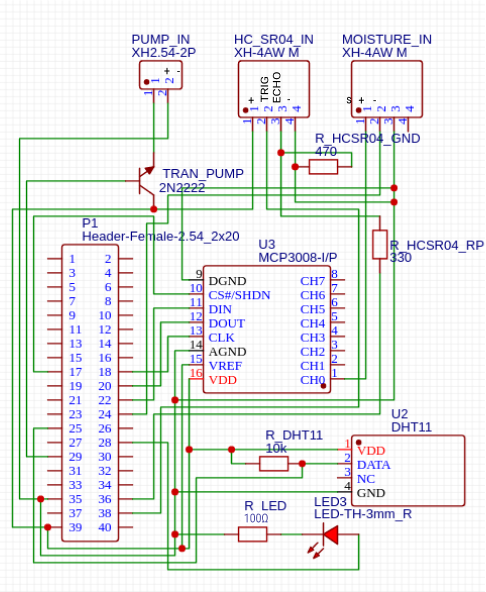
\includegraphics[width=\linewidth]{pcb.png}
		\caption*{Diagram PCB}
	\end{subfigure}
	\begin{subfigure}[b]{0.4\linewidth}
		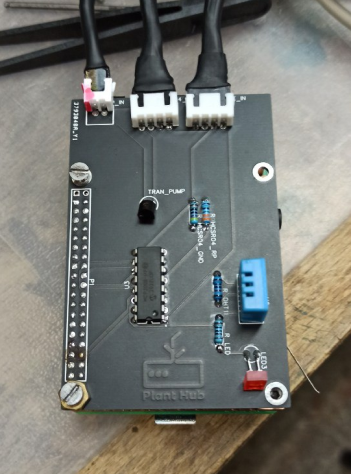
\includegraphics[width=\linewidth]{planthub.png}
		\caption*{PlantHub PCB se senzory}
	\end{subfigure}
\end{figure}

\section*{Hlavní program}

\subsection*{Postup práce}

Náš hlavní program pro zavlažování a komunikaci s databází a webovým rozhraním jsme začali psát ve vysokoúrovňovém programovacím jazyce python. Od toho jsme ale nakonec upustili kvůli vysokým technickým nárokům, což nám zpomalovalo průběh programu, proto jsme přešli na programovací jazyk GO.

\begin{figure}[h]
	\centering
	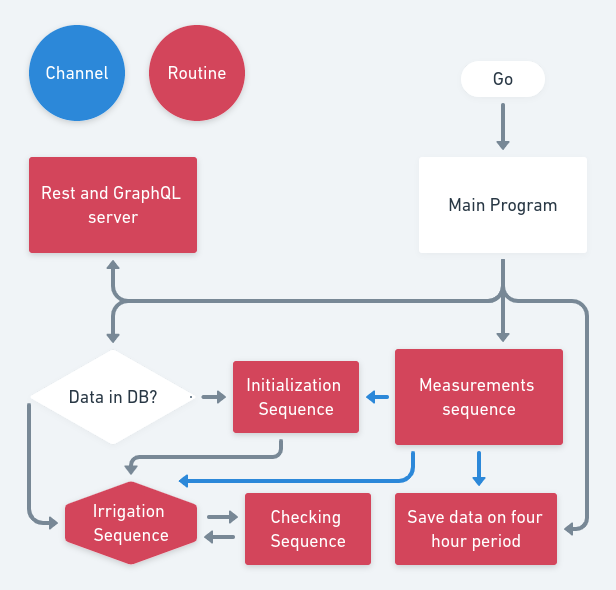
\includegraphics[width=8cm]{go.png}
	\caption*{Vývojový diagram programu}
\end{figure}

\subsection*{Fáze programu}

\subsubsection*{Inicializace}

Půda musí být ze začátku suchá. Senzor vlhkosti půdy zastrčíme co nejhlouběji do půdy. Rpi bude chvíli sbírat data a pak je zprůměruje do hodnoty, která bude sloužit jako limit pro spuštění čerpadla.

V UI jde navíc ještě manuálně nastavit hranice teploty a vlhkosti vzduchu pro spuštění čerpadla.

Nastavit se dá také množství vody, které bude přečerpáno při jednom spuštění a jaká je hranice pro přijatelnou výšku hladiny vody v nádrži. Pokud nejsou tyto hodnoty uvedeny čerpadlo bude vodu přečerpávat, dokud se nezmění hodnota kapacitního čidla pro měření vlhkosti půdy a HC-SR04 použije výchozí nastavení.

\subsubsection*{Měření}

Senzor vlhkosti půdy a DHT11 průběžně posílají naměřená data do Rpi, kde se ukládají do databáze. Jestliže naměřené hodnoty překročí limitní hodnoty, Rpi pošle signál pro otevření tranzistoru což spustí čerpadlo

\subsubsection*{Zavlažování}

Čerpadlo začne čerpat vodu a zavlažovat rostlinu. Voda se čerpá tak dlouho, dokud senzor vlhkosti půdy nezmění svou hodnotu nebo dokud není vyčerpán limit přečerpané vody na jedno spuštění.

\subsubsection*{Kontrola}

Po ukončení přečerpávání se spustí HC-SR04 a změří výšku hladiny vody. Naměřená data poté odešle do Rpi kde se uloží do databáze. Pokud bude naměřená hodnota nižší, než je limitní hodnota, začne blikat LED dioda a Rpi odešle upozornění o doplnění nádrže do UI. Jakmile bude hladina doplněna, signalizace se vypne.

\subsubsection*{Periodické ukládání dat}

V samostatné rutině běží funkce pro ukládání naměřených dat v periodě 4 hodin. Naměřená data jsou následně statisticky zobrazena v UI.

\subsubsection*{Ukládání dat}

Náš systém ukládá zvlášť periodicky naměřená data a data naměřená před zavlažováním, dále ukládá nastavení jak pro limity k zavlažování, tak pro webové rozhraní.

\section*{Webové rozhraní}

Webovovou aplikaci jsme napsali v JavaScriptovém frameworku React.js a css frameworku Tailwind. Ve webovém rozhraní je možné zobrazit si statisky jak živě naměřených dat, tak dat uložených v databázi. Z OpenWeather API získáváme data o předpovědi počasí.

\begin{figure}[h]
	\centering
	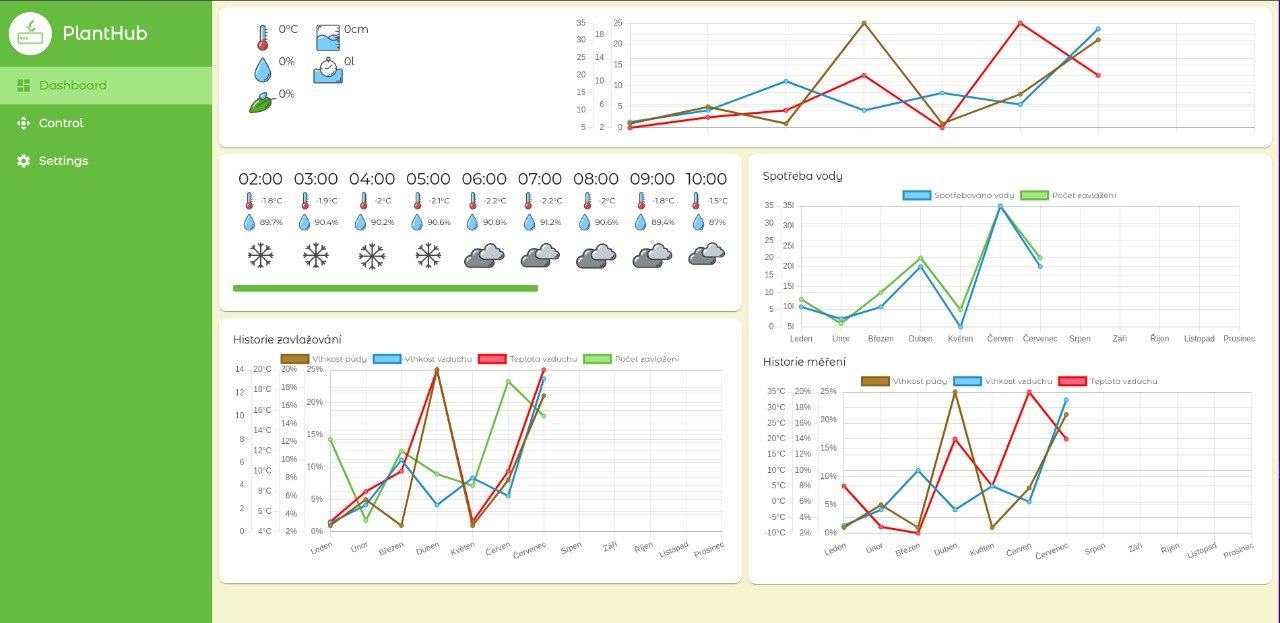
\includegraphics[width=\linewidth]{web-ui.png}
	\caption*{Uživatelské rozhraní}
\end{figure}

Interaktivní ovládání celého systému lze provést v již zmiňované webové aplikaci. Dovoluje uživateli kdykoliv spustit čerpadlo na zalévání rostliny.

\begin{figure}[h]
	\centering
	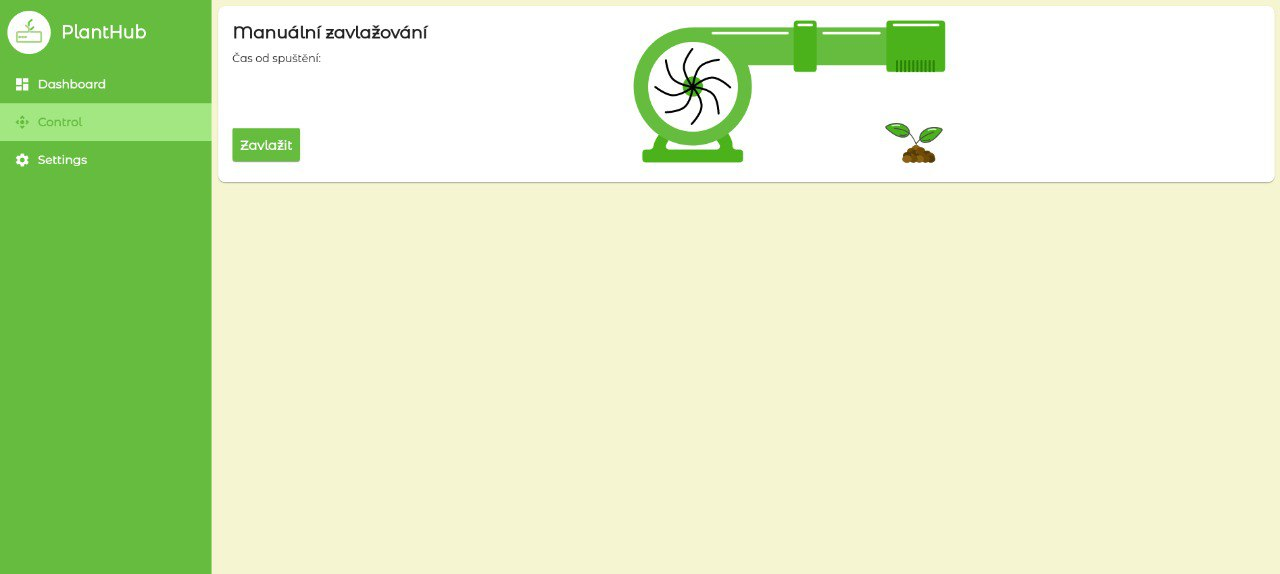
\includegraphics[width=\linewidth]{web-ui-pump.png}
	\caption*{Uživatelské rozhraní ovládání pumpy}
\end{figure}

V nastavení se dá změnit nastavení aplikace i limitů pro zavlažování. Data se po uložení uloží do databáze.

\begin{figure}[h]
	\centering
	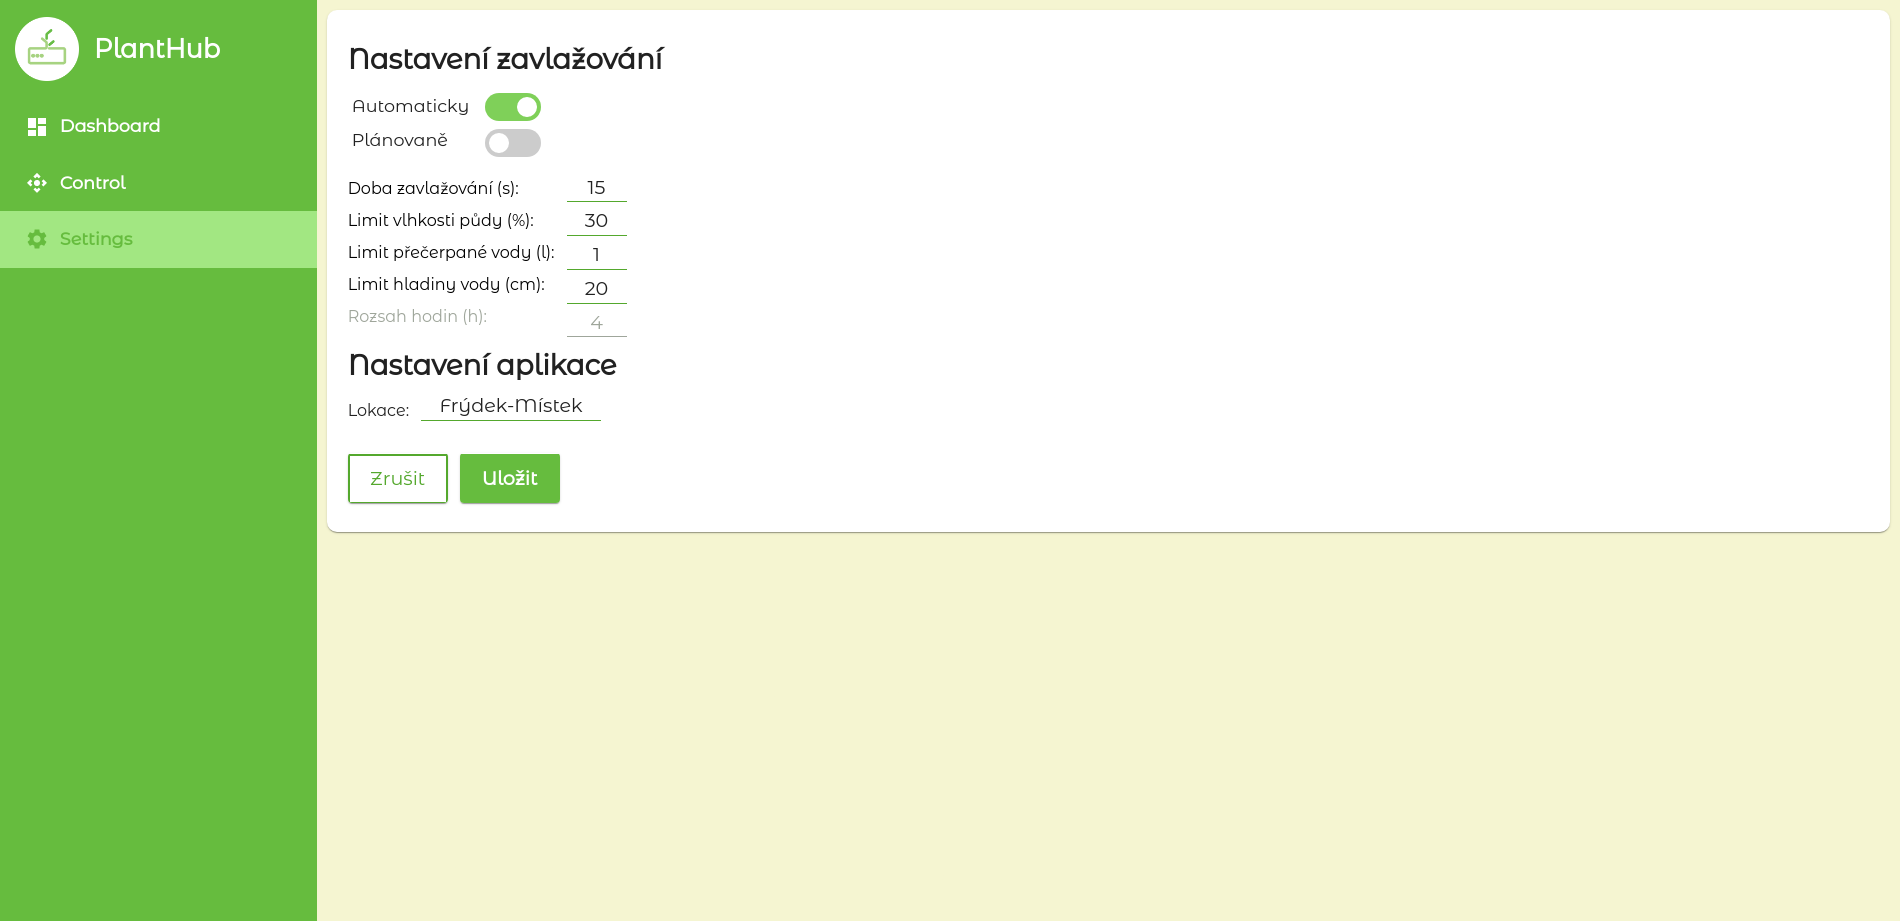
\includegraphics[width=\linewidth]{web-ui-settings.png}
	\caption*{Uživatelské nastavení}
\end{figure}

\section*{Databáze}

Pro databázi jsme se rozhodli použít databázový systém PostgreSQL. Jak vyplývá z názvu, jedná se o SQL databázi, ty jsou vhodné pro ukládání velkého objemu dat, jako právě data z našich senzorů. Webová aplikace používá pro přístup k datům z databáze GraphQL API.

GraphQL je query, který je konkurent řešení REST API. Nabízí efektivnější tvorbu API a také umožňuje efektivnější přístup k datům z databáze. Umožňuje vybrat pouze data, která momentálně aplikace používá a dovoluje vynechat data, která zrovna potřebné nejsou.

\section*{Webový server}

Web server jsme napsali v moderním jazyku Go, který nyní roste v popularitě hlavně mezi cloudovými vývojáři a v oblasti vývoje microservices. Dokáže se exekuční rychlostí přiblížit k nízkoúrovňovým jazykům jako je C nebo Rust, ale zároveň zůstává velmi lidsky čitelný a jednoduchý na použití. Na rozdíl od jazyků jako C a Rust má například garbage collector.

\section*{Seznam zkratek a pojmů}

\section*{Na čem ještě pracujeme}

- RPi case z 3D tisku
- Celková funkcionalita hlavního programu a jeho sekvencí
- Realizace nádrže pro vodu


\clearpage

\begin{acronym}
	\acro{API}{Application programming interface}
	\acro{REST}{Representaion programming interface}
	\acro{GraphQL}{Graph query languge}
	\acro{PCB}{Printed circuit board}
	\acro{RPi}{Raspberry Pi}
	\acro{ARM}{Advanced RISC Machines}
	\acro{GPIO}{General-purpose input/output}
	\acro{DHT11}{Digital humidity temperature (sensor) v.11}
	\acro{HC-SR04}{ltrasonický senzor vzdálenosti}
	\acro{MCP3008}{Analog-digital converter}
	\acro{Cerpadlo}{Ponorné mini čerpadlo eses}
	\acro{2N2222}{NPN tranzitor}
	\acro{SPI}{Serial peripheral interface}
\end{acronym}

\end{document}